\section{输入输出}
输入作为人与计算机之间最基本的交互方式,其中键盘和鼠标是标准输入设备。

CPU通过PIC\footnote{PIC通过中断控制请求使用CPU,即在需要的时候对CPU发出中断请求,暂停CPU现在运行的作业,先完成中断请求再继续之前的作业。}
(Programmable interrupt controller)与外部设备进行数据交换。
键盘作为计算机最早的外设,位于主PIC的IRQ1;
而鼠标作为第四代计算机才出现的输入设备,位于从PIC的IRQ12,而从PIC连接在主PIC的IRQ2。

输入设备工作时是将一个个指令\footnote{每一次敲击键盘按键,移动鼠标,点击鼠标都会产生相对应的指令。}
发送到CPU,而CPU同时只能处理一个指令(虽然处理时间非常短),用户输入的频率是无规律的\footnote{用户思考会暂停输入,而灵光闪现会加快输入。},
此时需要缓冲区fifo\footnote{缓冲区fifo采用先入先出的数据结构,使得先传入的输入指令能够率先得到执行。}接收输入数据并暂存,
在CPU处理完上一个输入时缓冲区向CPU传送下一个数据。缓冲区的作用是以协调输入和CPU之间的关系。

\subsection{缓冲区}

缓冲区数据结构参见程序~\ref{lst:fifo},运行流程如图~\ref{fig:fifo}所示。

\begin{figure}[H]
    \centering
    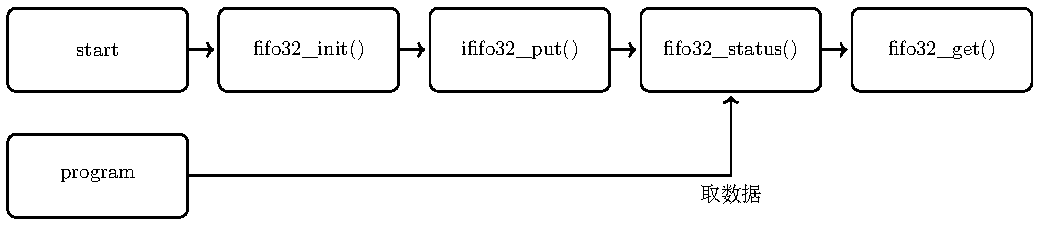
\includegraphics[width=\textwidth]{../Fig/func/fifo.pdf}
    \caption{缓冲区}
    \label{fig:fifo}
\end{figure}

\csingle|void fifo32_init(struct FIFO32 *fifo, int size, int *buf, struct TASK *task);|
\begin{itemize}
  \item 初始化缓冲区,设定缓冲区起始位置,读取位置,大小以及相关控制信息;
\end{itemize}

\csingle|int fifo32_put(struct FIFO32 *fifo, int data);|
\begin{itemize}
  \item 向FIFO写入数据并累积起来,及入栈一次;
\end{itemize}

\csingle|int fifo32_get(struct FIFO32 *fifo);|
\begin{itemize}
  \item 从FIFO取得一个数据,即出栈一次。\\
\end{itemize}

缓冲区在初始化 (fifo32\_init()) 成功后开始接受数据 (fifo32\_put());

程序调用接收数据需求 (fifo32\_get()) 时判断缓冲区 (fifo32\_status()) 不为空的情况下取出数据。
\begin{listing}[H]
  \inputminted[tabsize=2, firstline=40, lastline=44,
    linenos=true]{c}{../ZOS/src/kernel/bootpack.h}
  \caption{数据结构-缓冲区fifo}
  \label{lst:fifo}
\end{listing}
\begin{description}
\item[*buf:]缓冲区在内存中的地址;
\item[p, q:]下一个写入地址,下一个数据读入地址;
\item[size, free:]缓冲区大小,空闲空间大小;
\item[TASK flags:]溢出标记(-1和0分别表示有溢出和无溢出);
\item[TASK *task:]在当前位置释放内存。
\end{description}

操作系统运行后始终通过函数fifo32\_status(\&fifo)\footnote{存储总量 = size - free.}
监测fifo缓冲区内是否有数据,如果有数据才执行下一步对输入指令的响应。
接收输入信号的函数fifo32\_get(\&fifo)负责从缓冲区fifo中取出一个数据(键盘为1个字节,鼠标为4个字节)交由CPU处理。

流程如图~\ref{fig:fifo}所示,代码参见附录程序~\ref{lst:kbd1}和附录程序~\ref{lst:kbd2}所示。

% --------------------

\subsection{标准输入}
计算机收到数据后根据数据的大小区间区分这一段数据是何处传来的并进行相应处理。
一旦收到的指令为256到511,系统判定为键盘输入;
当指令为512到767,系统判定为鼠标输入。

输入流程如图~\ref{fig:io}所示。
\begin{figure}
  \centering
  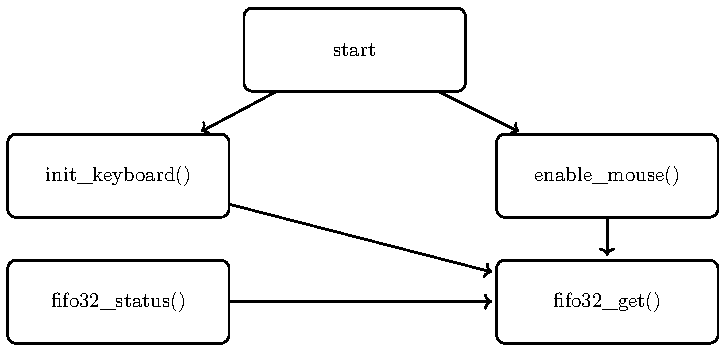
\includegraphics[width=.7\textwidth]{../Fig/func/io.pdf}
  \caption{标准输入}
  \label{fig:io}
\end{figure}

\csingle|init_keyboard(&fifo, 256);|
\begin{itemize}
  \item 将FIFO缓冲区的信息保存到全局变量里并初始化键盘控制器;
\end{itemize}

\csingle|void enable_mouse(struct FIFO32 *fifo, int data0, struct MOUSE_DEC *mdec);|
\begin{itemize}
  \item 将FIFO缓冲区的信息保存到全局变量里并激活鼠标。\\
\end{itemize}

操作系统启动后启用键盘输入(init\_keyboard())和鼠标输入(enable\_mouse())。

在缓冲区获得输入数据后,程序调用接收数据需求(fifo32\_get())后获得输入数据。

\subsubsection{键盘输入}

键盘作为最基础也是大众使用最精确的输入设备,它负担着很多的责任:
\begin{enumerate}
\item 输入文本按键
\item 修改文本输入的基本指令按键
\item 修改计算机的状态特殊按键
\end{enumerate}

按下不同的功能按键,键盘向计算机发送的指令是不一样的。

若输入指令为256-0x80+256时,为输入文本指令;

输入指令为退格键,回车键;

修改计算机的状态特殊按键如表~\ref{tab:spccmd}所示。
\begin{table}[!ht]
  \centering
  \begin{tabular}{lc|lc}
    \hline 功能 & 指令 & 功能 & 指令 \\
    \hline 左Shift & 256+0x2a & CapsLock & 256+0x3a \\ 
     右Shift & 256+0x36 & NumLock off & 256+0xaa \\
     左Shift off & 256+0xaa & ScrollLock & 256+0xaa \\
     右Shift off & 256+0xb6 & & \\
    \hline
  \end{tabular}
  \caption{修改状态的特殊指令}
  \label{tab:spccmd}
\end{table}

% ---------------------

\subsubsection{鼠标输入}

鼠标作为第四代计算机才出现的输入设备,因为涉及到坐标位置的变化,它的输入指令较键盘也相对复杂,
从鼠标传到计算机的信号都是4个字节一组的,其中第一个字节表示状态,其他3个有效指令分别为x坐标,y坐标以及鼠标按键状态。
根据鼠标接受数据的格式,数据结构设计参见程序~\ref{lst:mouse_data}。

\begin{listing}[H]
  \inputminted[tabsize=2, firstline=126, lastline=129,
    linenos=true]{c}{../ZOS/src/kernel/bootpack.h}
  \caption{数据结构-鼠标输入的数据}
  \label{lst:mouse_data}
\end{listing}
\begin{description}
\item[buf:]存放鼠标一个数据指令的数组;
\item[phase:]当前鼠标工作的阶段;
\item[x, y]缓冲区大小,空闲空间大小;
\item[btn]按键状态。
\end{description}

% ----------------------

\subsection{标准输出}

由于是面对硬件开发操作系统,无法使用各种成熟的库和函数,
所以输出也只能从修改VRAM的一个个像素开始。

流程如下:
通过一系列指令后,系统需要向屏幕打印字符,
则从数组中读取一个数据,并从字体库(包含基本字体的像素化数组)中找到对应的显示方法,
写入VRAM(Video RAM),在屏幕对应坐标范围内显示数据,
循环读取下一个并显示下一个数据。